\documentclass{article}[11pt]
% fancybox prevents the TOC from printing
%\usepackage{fancyhdr, fancybox, tabularx, verbatim, epsfig}
\usepackage{fancyhdr, tabularx, verbatim, epsfig}
\usepackage{amssymb,psboxit}
\usepackage{rotating}

\setlength{\oddsidemargin}{0.1\oddsidemargin}
\setlength{\evensidemargin}{0.5\evensidemargin}
\setlength{\topmargin}{0.0\topmargin}
\setlength{\textheight}{1.16\textheight}
\setlength{\textwidth}{1.35\textwidth}
\newcommand{\Aztec}  {{\sc Aztec}}
\newcommand{\Aztecoo}  {{\sc AztecOO}}
\newcommand{\aztecoo}  {{\Aztecoo}}
\newcommand{\epetra}  {{\sc Epetra}}
\newcommand{\epetraext}  {{\sc EpetraExt}}
\newcommand{\ML}     {{\sc ML}}
\newcommand{\trilinos}  {{\sc Trilinos}}
\newcommand{\amesos}  {{\sc Amesos}}
\newcommand{\meros}  {{\sc Meros}}
\newcommand{\anasazi}  {{\sc Anasazi}}
\newcommand{\umfpack}  {{\sc Umfpack}}
\newcommand{\superlu}  {{\sc SuperLU}}
\newcommand{\superludist}  {{\sc SuperLU\_dist}}
\newcommand{\mumps}  {{\sc Mumps}}
\newcommand{\klu}  {{\sc Klu}}
\newcommand{\metis}  {{\sc Metis}}
\newcommand{\parmetis}  {{\sc ParMetis}}
\newcommand{\triutils}  {{\sc Triutils}}
\newcommand{\ifpack}  {{\sc Ifpack}}
\newcommand{\parasails}  {{\sc ParaSails}}
\newcommand{\teuchos}  {{\sc Teuchos}}
\newcommand{\newpackage}  {{\sc new\_package}}
\newcommand{\zoltan}  {{\sc Zoltan}}
\newcommand{\nox}  {{\sc NOX}}
\newcommand{\loca}  {{\sc Loca}}
\newcommand{\MLAPI}  {{\sc MLAPI }}
\newcommand{\mlapi}  {{\sc MLAPI }}
\newcommand{\MLAPIns}  {{\sc MLAPI}}
\newcommand{\hypre}  {{\sc hypre}}
\newcommand{\petsc}  {{\sc PETSc}}
\newcommand{\be}  {\begin{enumerate}}
\newcommand{\ee}  {\end{enumerate}}
% Maxwell abbreviations
\newcommand \Ke {\ensuremath{K^{(e)}}}
\newcommand \Kn {\ensuremath{K^{(n)}}}
\newcommand \Th {\ensuremath{T_h}}
%\newcommand \curlcurl {({\it curl,curl})}
\newcommand \curlcurl {\ensuremath{\nabla\times\nabla\times}}

\newcommand{\comm}[2]{\bigskip
                      \begin{tabular}{|p{4.5in}|}\hline
                      \multicolumn{1}{|c|}{{\bf Comment by #1}}\\ \hline
                      #2\\ \hline
                      \end{tabular}\\
                      \bigskip
                     }
%
% ***********************************************************************
% * 02 July 1993: McCorkle                                              *
% * Define a macro that will lightly print the word `DRAFT' diagonally  *
% * across each page of the document. This macro was obtained from the  *
% * NMSU math department                                                *
% *                                                                     *
% * Usage: \draft                                                       *
% ***********************************************************************
%
\def\optionbox#1#2{\noindent$\hphantom{ii}${\parbox[t]{1.5in}{\it
#1}}{\parbox[t]{4.8in}{#2}} \\[1.1em]}

\def\choicebox#1#2{\noindent$\hphantom{th}$\parbox[t]{3.0in}{\sf
#1}\parbox[t]{3.35in}{#2}\\[0.8em]}

\def\structbox#1#2{\noindent$\hphantom{hix}${\parbox[t]{2.10in}{\it
#1}}{\parbox[t]{3.9in}{#2}} \\[.02cm]}

\def\protobox#1{\vspace{2em}{\flushleft{\bf Prototype}
\hrulefill}\flushleft{\fbox{\parbox[t]{6in}{\vspace{1em}{\sf
#1}\vspace{1em}}}}}


\def\draft{%
\special{!userdict begin /bop-hook{gsave
200 30 translate 65 rotate
/Times-Roman findfont 216 scalefont setfont
0 0 moveto 0.9 setgray (DRAFT) show grestore}def end}
}

\begin{document}
\bibliographystyle{siam}
\setcounter{page}{3}

\large

%\draft                                   % Lightly print `DRAFT' on every
                                         % page of the document

%
%
%\hspace{2.22in}
\begin{center}
SAND2005--1382 \\
%\hfill
%\hspace{2.41in}
Unlimited Release \\
%\hfill
%\begin{center}
Printed March 2005
\end{center}

\vspace{0.2in}

\begin{center}
{\Large {\bf \MLAPIns: A C++ Framework for Multilevel Preconditioners}}
%\footnote{ Sandia is a multiprogram laboratory operated by Sandia Corporation,
%a Lockheed Martin Company, for the United States Department of Energy's
%National Nuclear Security Administration under contract DE-AC04-94AL85000.}}}
%\footnote{ This work was supported by
%        the
%        Applied Mathematical Sciences program, U.S. Department of Energy,
%        Office of Energy Research, and was partially performed at 
%        Sandia National
%        Laboratories, operated for the U.S. Department of Energy under contract
%        No. DE-AC04-94AL85000.} }}

\vspace*{0.8in}
Marzio  Sala \\
Computational Math \& Algorithms \\
Sandia National Laboratories\\
P.O.~Box 5800 \\
Albuquerque, NM 87185-1110
\vspace*{1in}

\end{center}

\begin{abstract}
We discuss the design of \MLAPIns, an object oriented framework that enables
the development and usage of efficient, scalable and portable implementations
of multilevel preconditioners for general distributed sparse matrices, in both
serial and parallel environments. 

The main feature of this framework is the use of several programming paradigms
for the different implementation layes, with a strong emphasis on object
oriented classes and operator overloading for the top layer, and optimized
FORTRAN and C code for the layers underneath. In particular, \MLAPI takes
advantage of \ML~\cite{ml-guide}, the algebraic multilevel preconditioning
package of Trilinos~\cite{Trilinos-home-page}. 

\smallskip

In this paper, we 
outline the most important features of MLAPI, and we describe its usage
with several examples.

\bigskip

{\sl Note: An extended version of this paper, containing numerical comparisons
  between MLAPI and ML, has been submitted to ACM-TOMS.}
\end{abstract}

%
\clearpage
\newpage

\vfill
\begin{center}
(page intentionally left blank)
\end{center}
\clearpage
\newpage

\tableofcontents
\newpage

%-----------------------------------------------------------------------------%
\section{Introduction} 
\label{sec:introduction}
%-----------------------------------------------------------------------------%

The parallel solution of large linear systems of type
\begin{equation}
\label{eq:lin_sys}
A {x} = {b},
\end{equation}
where $A$ is a (distributed) large, real sparse matrix and $x$ and $b$ two real
multi-vectors, is the computational kernel of many applications. The solution
of such systems is a fundamental, and often the most time consuming,
  part of many simulation codes. Because of
the size of $A$, iterative solvers of Krylov type are generally
adopted~\cite{barret93templates}, the
best known methods being the conjugate gradient~\cite{hestenes52method} and
GMRES~\cite{saad86gmres}.
  
It is well known that the convergence of Krylov methods depends on 
the spectral properties of the linear system matrix
$A$~\cite{axelsson94iterative,saad96iterative,QSS}. Often, $A$ is very
ill-conditioned, so the
original system~(\ref{eq:lin_sys}) is replaced by
\[
P^{-1} A{u} = P^{-1} {b}
\]
(left-preconditioning), or by
\[
A P^{-1} P {u} = {b}
\]
(right-preconditioning), using a linear transformation $P^{-1}$,
called {\sl preconditioner}. $P^{-1}$ represents a sequence of operations
that somehow approximates the effect of $A^{-1}$ on a vector. 
Loosely stated, a preconditioner is any
kind of transformation applied to (\ref{eq:lin_sys}) which makes it
easier to solve, in terms of iterations and CPU time; see for
instance~\cite{greenbaum97iterative,golub97closer,vorst95parallel}. More precisely,
the general (and challenging) problem of finding an efficient
preconditioner is to identify a linear operator $P$ with the following
properties:
\begin{enumerate}
\item {\bf $P$ is a good approximation of $A$ is some sense}. Although no
  general theory is available, we can say that $P$ should act so that
  $P^{-1} A$ is near to being the identity matrix and its eigenvalues
  are clustered within a sufficiently small region of the complex plane;
\item {\bf $P$ is efficient}, in the sense that the iteration method converges
  much faster, in terms of CPU time, for the preconditioned system.  In
  other words, preconditioners must be selected in such a way that the
  cost of constructing and using them is offset by the improved
  convergence properties they permit to achieve;
\item {\bf $P$ or $P^{-1}$ can be constructed in parallel}, to take advantage of the architecture of modern supercomputers.
\end{enumerate}

\smallskip

A very successful class of preconditioners is represented by multilevel (or
multigrid) methods.
A multilevel method tries to approximate
the original PDE problem of interest on a hierarchy of grids and use
`solutions' from coarse grids to accelerate the convergence
on the finest grid.  
Multilevel and multigrid methods were introduced in the late 70's, and their
success and development is testified by the enormous literature and the several
international conferences organized since then. 
At least three
approaches have been presented in literature to define the multilevel
hierarchy:
to use a sequence of grids, as done in geometric multigrid~\cite{brandt.classic,hack.book,hack2.book}
to coarsen on each level by identifying a set of coarser-level nodes
(the so-called C-nodes) and finer-level nodes (F-nodes) 
(see for instance \cite{Briggs,WHackbusch_1985a}), or 
to coarsen on each level by grouping the nodes into contiguous subsets,
called aggregates, as done in smoothed 
aggregation~\cite{vanek1,vanek2,vanek3}.
Multilevel methods are well understood on model problems, while their
application to more general, non-symmetric, problems still requires
further developments.

\smallskip

\begin{figure}
\begin{center}
\begin{tabular}{ p{12cm} }
\hline
\vspace*{0.1cm}
\hspace*{1cm}
\begin{minipage}{10cm}
\begin{verbatim}
MultiLevelStartUp(A, MaxLevels, k)
{
  if (k == MaxLevels)
    return;
  else {
    P[k] = BuildP(); 
    R[k] = BuildR();
    A[k] = R[k] * A[k] * P[k];
  }
}
\end{verbatim}
\vspace*{0.1cm}
\end{minipage} \\
\hline
\end{tabular}
\caption{Pseudo-code of a the multilevel start-up procedure.}
\label{fig:startup}
\end{center}
\end{figure}

\begin{figure}
\begin{center}
\begin{tabular}{ p{12cm} }
\hline
\vspace*{0.1cm}
\hspace*{1cm}
\begin{minipage}{10cm}
\begin{verbatim}
MultiLevelSolve(A, f, x, k) 
{
  if (k == CoarsestLevel)
    u = CoarseSolver(A[k]), b);
  else {
    u = Smoother(A[k], f, u);
    r = R[k] * (f - A[k] * u);
    v = 0;
    MultiLevelSolve(A[k + 1], v, k + 1);
    u = u + P[k] * v;
    u = Smoother(A[k], f, u);
  }
}
\end{verbatim}
\vspace*{0.1cm}
\end{minipage} \\
\hline
\end{tabular}
\caption{Pseudo-code of a multilevel application procedure.}
\label{fig:application}
\end{center}
\end{figure}

Like most preconditioners, a multilevel preconditioner requires a startup 
procedure (a common version of which is reported in Figure~\ref{fig:startup})
  and an application procedure (reported in Figure~\ref{fig:application}).
In the Figures, \verb!k! is the current level,
\verb!A! is an array of matrices, with \verb!A[k]! the operator for 
level \verb!k! and \verb!A[0]! containing the matrix of the linear system 
(\ref{eq:lin_sys}), 
\verb!R[k]! is the restriction operator from level \verb!k! 
to level \verb!k + 1!, and \verb!P[k]! is the prolongator
operator from level \verb!k + 1! to level \verb!k!,
\verb!CoarseSolver()! is a generic direct solver, and
\verb!Smoother()! is a generic smoother (that is, an approximate solver
whose goal is to reduce the high frequencies of the error).

The effectiveness of the multilevel algorithm heavily depends on 
how the operators \verb!A[k], P[k], R[k]! are defined. To leverage software
development, it is preferable to code the multilevel preconditioner in a
general framework, based on abstract interfaces. Eventually, a  wide range
of preconditioners based on these abstract interfaces should be available so
that a method that matches the difficulty of the problem and the computational
architecture available can be adopted.

\smallskip

Note that two distinct sets of operations can be identified in the multilevel
procedures:
\begin{enumerate}
\item operations that require operators as unique identities (for example,
  the application of an operator, \verb!y = A * x!);
\item operations that require the specific knowledge of the structure
  of an operator and its internal data (for instance, the definition of the
  prologator operator \verb!P[k]!).
\end{enumerate}

Our aim is to simply the coding of a multilevel algorithm, by allowing
an intuitive syntax for all operations in group (1), and by condensing
operations in group (2) in well defined functions (or classes). 

Ideally, the code should not look too different from what we have just
presented, which in turn is just a modest change with respect to the
mathematical standpoint used to define a multilevel method. Unfortunately,
  this is not what happens in most codes.  Traditionally, coding is made
  complex by ``details'' inessential to the algorithm, like, for example, the
  dimension of the input and output vector, of flags for the smoother or the
  matrix-matrix product, or the parallel data layout.

Since these ``details'' are necessary to compile and run the program, our aim
is the following: {\em let the compiler take care of the details, and let the
  programmer-developer to focus on the algorithm}. For example, any well
  designed implementation of a linear operator already contains the number of
  rows and columns, and the implementation of a vector contains the number of
  elements in the vector.  By using a light layer of C++ and taking advantage
  of operator overloading (see, for example, \cite{stroustrup91cpp}), one can
  instruct the compiler on how to look for all the necessary information, so
  that all operations are properly executed.

\smallskip

In this paper, we want to show that it is possible to obtain intuitive,
  easy-to-read and easy-to-develop codes, that are {\sl at the same time}
  efficient and scalable.  This paper is organized as follows. First, in
  Section~\ref{sec:design} we will outline why an object-oriented interface
  can be useful to develop multilevel preconditioners (and, more general,
                                                       multilevel solvers).
  Section~\ref{sec:basic} introduces the most important \MLAPI classes, whose
  usage is presented in Section~\ref{sec:usage}. The
  MATLAB~\copyright~interface is detailed in Section~\ref{sec:matlab}.
  Section~\ref{sec:conclusions} outlines the conclusions.

%-----------------------------------------------------------------------------%
\section{Software Design}
\label{sec:design}
%-----------------------------------------------------------------------------%

We have defined the \MLAPI library to handle the definition of multilevel
preconditioners for sparse large linear systems of type (\ref{eq:lin_sys})
  on distributed memory computers.
Our aim was to design develop a general framework, that is portable and
straightforward to use, while being both flexible and efficient. 
The design of the library is based on the following principles:

\bigskip

\noindent
{\bf Portability.} Implementations of numerical algorithms should be
directly portable across machine platforms.
\MLAPI is written in ANSI C++. The STL library is
employed to increase efficiency. For message
passing, we adopted MPI, which is the {\em de-facto} standard, and as such
widely available and accepted by users of parallel applications. As a result,
  \mlapi has been successfully compiled on Linux, SGI Origin, DEC-alpha, SUN,
  and MAC OS X.

\bigskip

\noindent
{\bf Clarity.} Implementations of numerical algorithms should resemble
the mathematical formulation on which they are based. This is in contrast to
FORTRAN and C, which can require complicated subroutines or function calls,
  with a long parameter list.
A key design for \MLAPI was a user interface that is
intuitive. Our intention is that it should be possible for this
library to be used by those who have only a basic knowledge of MPI and C++.
Ideally, the structure of all \MLAPI kernels should be as close as possible to
the that of MATLAB. We have developed two types of C++ interfaces to basic
kernels. The first type utilizes the binary operators {\tt *, +, -},
  overloaded using the C++ capabilities. The second type is a set of
  interfaces (methods, functions) which can group triads or perform more
  complex operations.

\bigskip

\noindent
{\bf Flexibility.} \MLAPI is not based on any particular matrix format. This
is particularly convenient since several matrix formats are currently in used.
\MLAPI supports any data format that can offer a {\tt getrow()} function,
  which returns the column ID and the value of all nonzero elements for any
  locally hosted row. C users can provide this using the {\tt ML\_Operator}
  structure, while C++ users can derive a class from the pure virtual {\tt
    Epetra\_RowMatrix} class of the \epetra\ package.  Similarly, all operators defined by \MLAPI are
    wrapped as {\tt Epetra\_RowMatrix} and {\tt ML\_Operator}, so that users
    can access their nonzero elements without worrying about the actual data
    storage used by \MLAPI.
\bigskip

\noindent
{\bf Extensibility.} Multilevel algorithms are far from being completely
understood for all classes of problems. It is important for the multilevel
library to be easily extended, to validate new approaches. To that aim,
encapsulation is used to hide details in
specific classes. Besides, a set of function based on abstract interfaces
is provided, to generate the necessary multilevel operators. Polymorphism
allows the user to derive classes to implement new features.
All \MLAPI classes and methods automatically use a set of
default parameters, that can be tuned by specifying the
desired parameters in a parameter list.

\bigskip

\noindent
{\bf High performance.} A good numerical package that utilizes OO programming
must exhibit a computational efficiency that is comparable to that of FORTRAN
and C codes. This puts severe limitations to the OO design. It is certain easy
to generate elegant but inefficient C++ code.  We implemented \MLAPI as a
light layer of C++, on the top of
a mixture of FORTRAN77 kernels (BLAS~\cite{dongarra90set} and
                                LAPACK~\cite{demmel89lapack}) 
for all dense matrix
operations and vector updates, C functions for all sparse matrix operations
(like distributed sparse matrix-matrix product), and C++, for memory
management. The layer
structure of \MLAPI is shown in Figure~\ref{fig:layer}. Lower layers of the
library indicates an encapsulation relationship with upper layers. As a
result, \MLAPI is (almost) as
efficient as the C or FORTRAN library underneath.

\begin{figure}
\begin{center}
\includegraphics[width=12cm]{layer.eps}
\caption{Layer structure of \MLAPI.}
\label{fig:layer}
\end{center}
\end{figure}

\bigskip

\noindent
{\bf Memory Management.} One of the most powerful feature of C and C++
if the capability of allocating memory. Unfortunately, this is also the
area where most bugs are found -- not to mention memory leaks. We have adopted
smart pointers to manage memory~\cite{barlett04teuchos}.
\MLAPI objects should never be allocated using {\tt new}, and therefore never
free them using {\tt delete}. The code automatically deletes memory
when it is no longer referenced by any object. Besides, functions or methods
that need to return \MLAPI objects, should always return an instance of the
required object, and not a pointer or a reference.

\noindent
At a first glance, this may appear as a major limitation for optimal
performances. Dealing with an instance of an object, and not with pointers or
references, signifies that the new instances have to be created and copied,
usually an expensive operation. This is {\sl not} what happens with \MLAPIns. In
fact, all \MLAPI objects are defined as light containers of pointers,
  automatically allocated and managed as necessary. 
%  For
%example, a {\tt MultiVector} (introduced in Section~\ref{sec:multivector})
%  needs to store a pointer to the double array
%containing the vector elements. When memory is allocated within an \MLAPI
%object, this is done using the so-called smart pointers, or self-counting
%pointers\footnote{\MLAPI uses the RefCountPtr or the \teuchos~package to 
%manage memory. We refer to the Teuchos web page for more details.}.

\noindent
Let us consider three generic \MLAPI objects.
The assignment \verb!A = B! means the following: all smart pointers contained
by \verb!B! are copied in \verb!A!, both \verb!A! and \verb!B! point to the
same memory location. However, \verb!A! and \verb!B! are not aliases: we can
still write \verb!B = C!, meaning that \verb!A! contains what was contained in
\verb!B!, and both \verb!B! and \verb!C! point to the same memory location. 
Should we need to create a copy of \verb!C! in \verb!B!, we will use the
instruction \verb!B = Duplicate(C)!, which is instead an expensive operation, as new memory
needs to be allocated, then all elements in \verb!C! need to be copied in
\verb!B!.

\medskip

\noindent
{\bf Operator overloading.} Operator overloading is an 
interesting capability of C++ that has been only
partially used in the scientific computing community. We adopt expression
templates (see for instance~\cite{vandevoorde03cpp}) to increase the
performances of MLAPI.

%-----------------------------------------------------------------------------%
\section{\MLAPI Classes}
\label{sec:basic}
%-----------------------------------------------------------------------------%

In this section we introduce the
most important classes of \MLAPI: {\tt Space} 
(analyzed in Section~\ref{sec:space}), {\tt MultiVector}
(analyzed in Section~\ref{sec:multivector}),
{\tt Operator} (described in Section~\ref{sec:operator}) and 
{\tt InverseOperator} (in Section~\ref{sec:inverseoperator}). Furthermore,
\MLAPI furnishes two matrices classes, {\tt SerialMatrix} and 
{\tt
  DistributedMatrix}, to set the matrix elements in a very intuitive 
  way.

The inheritance diagram is reported in Figure~\ref{fig:in}. All classes are
derived from a basic class, {\tt BaseObject}. Entities that are mathematically
equivalent to operators are derived from {\tt BaseOperator} class, which
basically contains only method {\tt Apply()}. Two concrete implementations are
{\tt Operator} and {\tt InverseOperator}.  Classes {\tt Operator}, {\tt
  InverseOperator}, {\tt MultiVector} all derived also from {\tt CompObject}
  and {\tt TimeObject}. These two classes, not  described here, are used to
  count flops and track the time spent in given methods. 

\begin{figure}
\begin{center}
\includegraphics[width=12cm]{MLAPI_classes.eps}
\caption{Inheritance diagram for \MLAPI classes.}
\label{fig:in}
\end{center}
\end{figure}

We note that \MLAPI preconditioners can be easily wrapped as \epetra\ objects,
  and therefore used by any library of application that understand \epetra\
  (for example, Krylov accelerators such as \aztecoo, eigensolvers such as
   \anasazi, physics-based preconditioners as \meros, and the \trilinos\ API,
   TSF).

%-----------------------------------------------------------------------------%
\subsection{The {\tt Space} Class}
\label{sec:space}
%-----------------------------------------------------------------------------%

A {\tt Space} is the fundamental \MLAPI class. All distributed objects must have
underlying spaces, which define the global dimension of the object 
(for example, the total number of elements in a vector) as well as the
 parallel layout (i.e., the distribution of these elements across the
processors). The easiest way to define a {\tt Space} is by specifying the
number of global elements 
and/or the number of local elements,
\begin{verbatim}
int NumGlobalElements = 128;
int NumLocalElements  = 16;
Space S(NumGlobalElements);
Space S2(-1,NumLocalElements);
\end{verbatim}
In both cases, a linear distribution is implicitly 
assumed\footnote{That is, processor 0 hosts all elements with a global ID
  from 0 to {\tt NumLocalElements - 1}, processor 1 from {\tt
    NumLocalElements} to {\tt 2 * NumLocalElements - 1}, etc.}. If a non-linear
distribution is required, one can simply write
\begin{verbatim}
int NumMyElements = 128;
int* MyGlobalElements;
// define here MyGlobalElements
Space S1(-1,NumMyElements,MyGlobalElements);
\end{verbatim}
where {\tt MyGlobalElements[i]} is the global ID or local node {\tt i}.

The global ID of local node {\tt i} is returned using the operator ():
\begin{verbatim}
int LID = 2;
int GID = S(LID);
\end{verbatim}

\smallskip

As all memory is managed using smart pointers, the users can let a object go
out scope even if this object has been used to define new objects. This is
typically the case with {\tt Space}'s. Let us consider the following function:
\begin{verbatim}
MultiVector foo(int NumGlobalElements)
{
  Space S(NumGlobalElements);
  MultiVector V(S);
  // do something on V, for example set all elements to 1.0
  V = 1.0;
  return(V)
}
\end{verbatim}
Clearly, object {\tt S} will go out of scope after returning from {\tt foo}.
However, the code will do the following: as {\tt V} is created, a {\tt Space}
object, say {\tt V2}, is defined within {\tt V}, so that {\tt V2 = V}
(light-weight copy). All smart pointers in {\tt V} are copied within {\tt V2},
and {\tt V} can go out of scope without damaging the returned vector 
(and without memory leaks).

%-----------------------------------------------------------------------------%
\subsection{The {\tt MultiVector} Class}
\label{sec:multivector}
%-----------------------------------------------------------------------------%

{\tt MultiVector}'s are the \MLAPI class for distributed double-precision
vectors. Once a space (say, {\tt S}) has been defined, vectors can be created
as
\begin{verbatim}
MultiVector x(S), y(S); // specify the space in ctor...
MultiVector z;          // ... or create empty vector
\end{verbatim}

The number of local elements in a vector is returned by method {\tt
  GetMyLength()}, and the global number of elements by
{\tt GetGlobalLength()}. To set all the elements of a {\tt MultiVector} to the same value, say 2, simply type {\tt x = 2.0}. To modify a given (local) element, one can proceed as follows:
\begin{verbatim}
for (int i = 0 ; i < y.GetMyLength() ; ++i)
  y(i) = 1.0 * x(i);
\end{verbatim}
that is, a reference to the $i-$element of the vector is returned using
operator \verb!()!.  The sum of two vectors is simply
\begin{verbatim}
z = x + y; z = 2.0 * x - 3.0 * y; 
\end{verbatim}
The scalar product between {\tt x} and {\tt y} is {\tt x * y}. The 2-norm is
returned by method {\tt Norm2()}; {\tt Random()} populates the vector with
random values; {\tt Reciprocal()} replaces each element with its inverse. 
Method {\tt GetValues()} returns the pointer to the internally stored double
array. Note
that efficient BLAS functions are used for copy and DAXPY operations. 

\smallskip

Often, it is necessary to define a set of vectors, all sharing the same space.
This can be obtained as follows:
\begin{verbatim}
int NumVectors = 3;
MultiVector w(S,NumVectors);
w.Random();
for (int i = 0 ; i < w.GetMyLength() ; ++i)
  for (int j = 0 ; j < w.GetNumVectors() ; ++j)
    cout << w(i,j) << endl;
\end{verbatim}
All vectors in a multivector are stored in the same double array,
  consecutively.

\smallskip

It is also possible to create a {\tt MultiVector} by providing an already
allocated double array:
\begin{verbatim}
Space S(-1, NumMyElements);
double* ptr = new double[NumMyElements];
// here populate ptr as necessary
MultiVector v(S, ptr, ownership);
assert (v(i) == ptr[i]);
\end{verbatim} 
By setting parameter {\tt ownership} to {\tt true}, then {\tt V} will take
care of deleting memory when no objects refer to it\footnote{It is supposed
  that {\tt ptr} has been allocated using {\tt new}.}. By setting {\tt
  ownership} to {\tt false}, instead, the user will take care of deleting {\tt
    ptr}.

%-----------------------------------------------------------------------------%
\subsection{The {\tt Operator} Class}
\label{sec:operator}
%-----------------------------------------------------------------------------%

An {\tt Operator} is a (linear or nonlinear) map between two {\tt Space}'s, the
domain space and the range space. An {\tt Operator} object can be created
by passing a pointer to an already {\tt FillComplete()}'d {\tt
Epetra\_RowMatrix},
\begin{verbatim}
Epetra_RowMatrix* Epetra_A;
// create and FillComplete() here Epetra_A
Operator A(DomainSpace, RangeSpace, Epetra_A, ownership);
\end{verbatim}
or by passing a pointer to an {\tt ML\_Operator} struct:
\begin{verbatim}
ML_Operator* ML_A;
// create and populate here ML_A
Operator A(DomainSpace, RangeSpace, ML_A, ownership);
\end{verbatim}
Finally, {\tt Operator}'s can be defined 
by manipulating already existing objects. If {\tt A} and {\tt B} are two
existing {\tt Operator} objects with suitable spaces, a new {\tt Operator C}
can be defined, for example, as {\tt C = A
+ B}, {\tt C = 1.0 * A + 3.0 * B}, {\tt C = A * B}. For the particular case of
triple matrix-matrix product, one can write {\tt D = GetRAP (A, B, C)}.
%

As \ML, \MLAPI is not based on any
particular matrix format. Rather, its matrix interface basically requires only
a capability to query for the nonzero elements in a given local row.
Therefore, it is easy to interface a given application with \MLAPIns.

\smallskip

An {\tt Operator} can be applied to a {\tt MultiVector},
\begin{verbatim}
Space DomainSpace(5);
Space RangeSpace(5);
MultiVector x(DomainSpace); x = 2;
MultiVector y(RangeSpace);
Operator I = Identity(DomainSpace, RangeSpace);
y = I * x;
\end{verbatim}

\smallskip

For a symmetric positive definite matrix, the A-norm of a vector can simply be
defined as \verb!sqrt(z * (A * z))!.
Some basic operations on matrices are also supported. For example,
one can extract the diagonal of a matrix as a vector, then create a new
matrix, containing this vector on the diagonal
\begin{verbatim}    
// A is an Operator
MultiVector z = GetDiagonal(A);
Operator D = GetDiagonal(z);
\end{verbatim}

Function {\tt Eig()} can be used to compute the eigenvalues of an
{\tt Operator}
(for serial runs only). This function calls LAPACK, therefore the
{\tt Operator} should be ``small''.
\begin{verbatim}    
MultiVector ER, EI, V;
Eig(A, ER, EI, V);

for (int i = 0 ; i < ER.GetMyLength() ; ++i)
  for (int j = 0 ; j < ER.GetNumVectors() ; ++j)
    cout << "ER(" << i << ", " << j << ") = " << ER(i,j) << endl;
\end{verbatim}

%-----------------------------------------------------------------------------%
\subsection{The {\tt InverseOperator} Class}
\label{sec:inverseoperator}
%-----------------------------------------------------------------------------%

A {\tt InverseOperator} is a (linear or nonlinear) map between two spaces, the
domain space and the range space, whose application to a given {\tt
  MultiVector} is meant to approximate the action of a given {\tt Operator}.
The most important difference between an {\tt Operator} and an {\tt
  InverseOperator} is that the latter has no definition of nonzero
  structure of matrix elements, while {\tt Operator} does. The only mathematical method implemented
  by {\tt InverseOperator} is {\tt Apply()}.

{\tt InverseOperator}'s usually define smoothers and coarse solvers in a
multilevel preconditioner. At present, point relaxation smoothers (of Jacobi,
Gauss-Seidel and symmetric Gauss-Seidel), several incomplete factorizations
and a complete LU factorization can be used as smoothers and coarse solver. A
simple example of usage here follows:
\begin{verbatim}
Operator A; // define the elements of A
Teuchos::ParameterList List;
List.set("smoother: sweeps", 2); 
List.set("smoother: damping factor", 0.67);
InverseOperator invA(A, "symmetric Gauss-Seidel",List);
\end{verbatim}
where 2 and 0.67 are the number of sweeps and the damping factor,
  respectively. A coarse solver can be defined as
\begin{verbatim}
InverseOperator coarse(A, "Amesos-KLU");
\end{verbatim}
which means that the KLU solver of \amesos\ will be adopted to compute the LU
factorization.

To apply the inverse of A using LU factorization one can write
\begin{verbatim}
InverseOperator invA(A,"Amesos-KLU");
\end{verbatim}
To verify that $x = A^{-1} A x$,
\begin{verbatim}
x = invA * (A * x) - x;
double NormX = sqrt(x * x);
\end{verbatim}

%-----------------------------------------------------------------------------%
\subsection{The {\tt SerialMatrix} and {\tt DistributedMatrix} Classes}
\label{sec:matrices}
%-----------------------------------------------------------------------------%

\MLAPI offers two convenient matrix classes, one for serial
computations only, and the other for serial or parallel computations. Both are
derived from the {\tt Operator} class, and overload the {\tt ()} operator to
facilitate the insertion and modification of elements.
The first class is
{\tt SerialMatrix}. An example of code to
create a tridiagonal matrix is as follows:
\begin{verbatim}
Space S(n); // n is the size of the matrix
SerialMatrix A(S, S);
for (int i = 0 ; i < n ; ++i) {
  A(i,i) = 2.0;
  if (i)          A(i, i - 1) = -1.0;
  if (i != n - 1) A(i, i + 1) = -1.0;
}
\end{verbatim}
The second class, {\tt DistributedMatrix} can be used to create distributed
matrices. Using this class, any process can set {\sl any} element of the
matrix (that is, both elements in the locally hosted rows, as well as elements
        hosted by another process). The following example creates a
distributed tridiagonal matrix:
\begin{verbatim}
Space S(n); // n is the global size of the matrix
DistributedMatrix A(S, S);

// loop over all local elements
for (int i = 0 ; i < S.GetNumMyElements() ; ++i) {
  int j = S(i); // get global ID of local element i
  A(j, j) = 2.0;
  if (j)          A(j, j - 1) = -1.0;
  if (j != n - 1) A(j, j + 1) = -1.0;
}
\end{verbatim}
After the insertion of all elements, the matrix structure must be ``freezed''
by calling method {\tt FillComplete()}. This method computes the data
structures required by the (distributed) matrix-vector product.  Matrix
elements cannot be added after the call to {\tt FillComplete()}; though, the
value of already existing elements can be modified.

By using the {\tt SerialMatrix} class, the user can insert matrix elements at
any time; however, the matrix-vector product has not been optimized. The {\tt
  DistributedMatrix} class, instead, offers an optimized matrix-vector
  product, since the matrix is internally stored by using the Epetra library.

%-----------------------------------------------------------------------------%
\section{Using \MLAPI}
\label{sec:usage}
%-----------------------------------------------------------------------------%

This section briefly explain how to use \MLAPIns\footnote{Compilable codes
can be found in {\tt ml/examples/MLAPI}.}. We also refer to the Doxygen
documentation for more details.

%-----------------------------------------------------------------------------%
\subsection{Initialize and Finalize the \MLAPI Workspace}
\label{sec:workspace}
%-----------------------------------------------------------------------------%

First, we need to initialize the \MLAPI workspace, using {\tt Init()} 
(which is automatically called by \MLAPI is the user forgets to do so). The
workspace should be cleaned using {\tt Finalize()} to avoid memory leaks.

All \MLAPI commands should be inserted
in a {\tt try/catch} block:
\begin{verbatim}
try {
  ... // here MLAPI stuff
}
catch (const int e) {
  cout << "Integer exception, code = " << e << endl;
} 
catch (...) {
  cout << "problems here..." << endl;
}
\end{verbatim}

%-----------------------------------------------------------------------------%
\subsection{Defining two-level Preconditioners}
\label{sec:two-level}
%-----------------------------------------------------------------------------%

We now present how to define a 2-level additive
preconditioner. Let {\tt A} be the fine-level matrix.
{\tt C}  the coarse level matrix,
and {\tt FineSolver} and {\tt CoarseSolver} 
the fine level smoother and the coarse level solver,
respectively. Let {\tt P} be the prolongator from the coarse space to the fine
space\footnote{As \MLAPI is based on ML, the user can easily build a
  prolongator operator based on smoothed aggregation process.}, then {\tt R}
  is the transpose of {\tt P}, and Galerkin projection is used to define {\tt
    C}:
\begin{verbatim}
Operator A, C, P, R;
// define here A and P
R = GetTranspose(P);
C = GetRAP(R,A,P);
\end{verbatim} 
We will use symmetric Gauss-Seidel
for the fine level, and LU for the coarse level:
\begin{verbatim}
InverseOperator FineSolver, CoarseSolver;
FineSolver.Reshape(A,"symmetric Gauss-Seidel");
CoarseSolver.Reshape(C,"Amesos-KLU");
\end{verbatim}
The application of the preconditioner will read as follows:
\begin{verbatim}
void foo(MultiVector& b_f, MultiVector& x_f)
{
  x_f = FineSolver(b_f);     // smoother
  r_c = R * r_f;             // restriction to coarse
  r_c = CoarseSolver_ * r_c; // solver coarse problem
  x_f = x_f + P * r_c;       // sum correction
}
\end{verbatim}

%-----------------------------------------------------------------------------%
\subsection{Writing \MLAPI Objects in MATLAB Format}
\label{sec:matlab}
%-----------------------------------------------------------------------------%

It is often convenient to use MATLAB to analyze matrices and
vectors. Distributed \MLAPI objects can dumped to a single, MATLAB compatible
ASCII file, by using class {\tt MATLABStream}.
Note that both serial and distributed objects 
are saved in just one file, which will contain the global object
(for example, a distributed matrix will be dumped using global row and
 column ordering). {\tt MATLABStream} behaves like a ``normal'' 
stream.  Objects can be saved in file by using the operator \verb!<<!.

Let {\tt S, V}, and {\tt A} be a {\tt Space}, a {\tt MultiVector}
and an {\tt Operator}. First, we have to define a {\tt MATLABStream} object by specifying the
file name,
\begin{verbatim}
MATLABStream matlab("mlapi.m");
\end{verbatim}
Then, we specify the label of each operator, as this
label will be used to define the name of the object in the output file,
\begin{verbatim}
S.SetLabel("S");
V.SetLabel("V");
A.SetLabel("A");
\end{verbatim}
Finally, we can simply write
\begin{verbatim}
matlab << "% a string comment is allowed\n";
matlab << S;
matlab << V;
matlab << A;
\end{verbatim}
We can also mix objects with MATLAB commands,
\begin{verbatim}
matlab << "plot(eig(A))\n";
\end{verbatim}
The output file is automatically closed. Note that it is not possible to write
on file an {\tt InverseOperator} object, as this class only defines the
action of the inverse of an operator on a given vector.

%-----------------------------------------------------------------------------%
\section{Concluding Remarks}
\label{sec:conclusions}
%-----------------------------------------------------------------------------%

Using C++ can greatly enhance clarity, reuse, and portability of numerical
libraries. In our C++  library, \MLAPIns, the implementation details are
completely hidden at the algorithm level, so that the resulting code greatly
resemble the algorithm itself. This object oriented framework is based on a
carefully designed set of classes and operator overloading, and allows the
algorithm developer to write a parallel, efficient (C++) code in a MATLAB-like
style. Operations on \MLAPI classes are then automatically translated by a
(standard) compiler into efficient code.  The advantage of this approach is
that the developer can focus on the algorithm itself, without spending time on
details that can be fixed by the compiler. This reduces the time spent in
writing and debugging the algorithm, at the only expense of a minimal increase
in the CPU time. We believe that this is a negligible factor in the
development and testing of new ideas, especially considering the time saved by
the developer to write the code itself. 

%-----------------------------------------------------------------------------%
\section*{Acknowledgments}
\label{sec:acks}
%-----------------------------------------------------------------------------%

We thank all the \ML\ developers, since \MLAPI could not exist without \ML, and
could not be efficient and flexible if \ML\ would not be so. \MLAPI also
relies of several other \trilinos~\cite{Trilinos-home-page} packages:
\epetra~\cite{epetra-guide}, \ifpack~\cite{ifpack-guide},
  \amesos~\cite{amesos-guide}, \teuchos, \aztecoo\ and \triutils. 

%-----------------------------------------------------------------------------%
\bibliography{MLAPI}
%-----------------------------------------------------------------------------%

\end{document}
